\section{量子位、量子门、量子线路}
\subsection{量子位}
比特是所有计算的基础。无论是录制数字视频、制作 3D 模型动画还是使用计算器应用程序,从操作系统到软件的所有数据均由二进制代码构建,二进制代码是比特的集合。计算机字节由八个比特组成,这是使用二进制表达一个文本字符所需的最少比特数。任意\textbf{两级系统},如果系统的状态只能是两个状态之一(例如,上或下,左或右,打开或关闭),均可用于表示一个比特。

在传统或经典计算中,可以将单个比特视为一段二进制信息,表示为 0 或 1。现代计算机里比特通常由电压或电流脉冲(或触发器电路的状态)表示。当这些系统中没有电流流动时,可将电路视为关闭,此状态表示为 0。当有电流流动时,可将电路视为开启,此状态表示为 1。

与经典位不同,量子位编码在量子态上,由于态的叠加性,除了0或1之外,它还可能处于0与1的叠加态。

\begin{define}{量子位(Quantum bit)}
在量子信息理论中,量子位(Qubit)是量子信息的基本单位,类似于经典计算中的比特(Bit)。然而,量子位与经典比特有着本质的不同。经典比特只有两种状态:0 和 1,而量子位可以同时处于 0 和 1 的叠加态。量子位是一个量子系统,其中布尔状态 0 和 1 由一对归一化且相互正交的量子基态表示。

 数学上,量子位的状态可以表示为:
     \[
     |\psi\rangle = \alpha |0\rangle + \beta |1\rangle
     \]
其中,\(\alpha\) 和 \(\beta\) 是复数,满足归一化条件:
     \[
     |\alpha|^2 + |\beta|^2 = 1
     \]
\(\alpha\) 和 \(\beta\) 分别表示量子位处于状态 \(|0\rangle\) 和 \(|1\rangle\) 的概率幅。
\end{define}
量子位可以由任何具有量子现象的粒子、亚粒子或准粒子实现。例如,超导量子位、离子阱量子位、拓扑量子位和光量子位等。这些物理系统可以实现量子位的初始化、操作和测量。

量子位可以处于任意的叠加态,这使得量子计算能够进行并行计算。例如,一个量子位可以处于:
     \[
     |\psi\rangle = \alpha|0\rangle + \beta |1\rangle
     \]
测量量子位时,其状态会坍缩为 0 或 1,概率分别为 \(|\alpha|^2\) 和 \(|\beta|^2\)。

 多个量子位可以形成量子纠缠态,这种状态下,量子位之间的状态不再是独立的,而是相互关联的。例如,两个量子位可以形成Bell态:
     \[
     |\Phi^+\rangle = \frac{1}{\sqrt{2}} (|00\rangle + |11\rangle)
     \]
在这种纠缠态下,测量其中一个量子位的状态会立即确定另一个量子位的状态,无论它们相距多远。

量子位的状态可以几何地表示为Bloch球上的一个点。Bloch球是一个单位球,其表面的点对应于量子位的所有可能状态。量子位的状态可以表示为:
     \[
     |\psi\rangle = \cos\left(\frac{\theta}{2}\right) |0\rangle + e^{i\phi} \sin\left(\frac{\theta}{2}\right) |1\rangle
     \]
其中,\(\theta\) 和 \(\phi\) 分别是极角和方位角。

量子位是量子计算的基本信息单元,具有量子叠加和量子纠缠的特性。通过数学表示,量子位的状态可以用二维复数向量描述,满足归一化条件。量子位的物理实现方式多样,包括超导量子位、离子阱量子位、拓扑量子位和光量子位等。量子位的测量是一个随机过程,测量结果会使其状态坍缩到 0 或 1。这些特性使得量子位在量子计算中具有巨大的潜力和应用价值。

\subsection{量子门}
量子门(Quantum Gate)是量子计算中的基本操作单元,通过幺正矩阵表示的线性变换改变量子位的状态。量子门是可逆的,可以组合成复杂的量子线路,实现量子算法。常见的量子门包括Hadamard门、Pauli-X门、Pauli-Y门、Pauli-Z门和CNOT门等。这些量子门在量子计算中具有重要的作用,是实现量子算法的基础。
\begin{define}{量子门(Quantum Gate)}
     量子门是量子计算中的基本操作单元,类似于经典计算中的逻辑门。量子门通过对量子位进行线性变换来改变其状态。量子门是可逆的,这意味着每个量子门都有一个逆门。

     量子门可以用一个幺正矩阵(Unitary Matrix)表示。对于一个作用在单个量子位上的量子门,其矩阵表示为一个 2x2 的幺正矩阵 \(U\),满足 \(U^\dagger U = I\),其中 \(U^\dagger\) 是 \(U\) 的共轭转置,\(I\) 是单位矩阵。矩阵的幺正性满足变换后态保持归一化。
\end{define}

\subsubsection{一位门}
\begin{figure}[htbp]
     \centering
     \caption{一位量子门}
     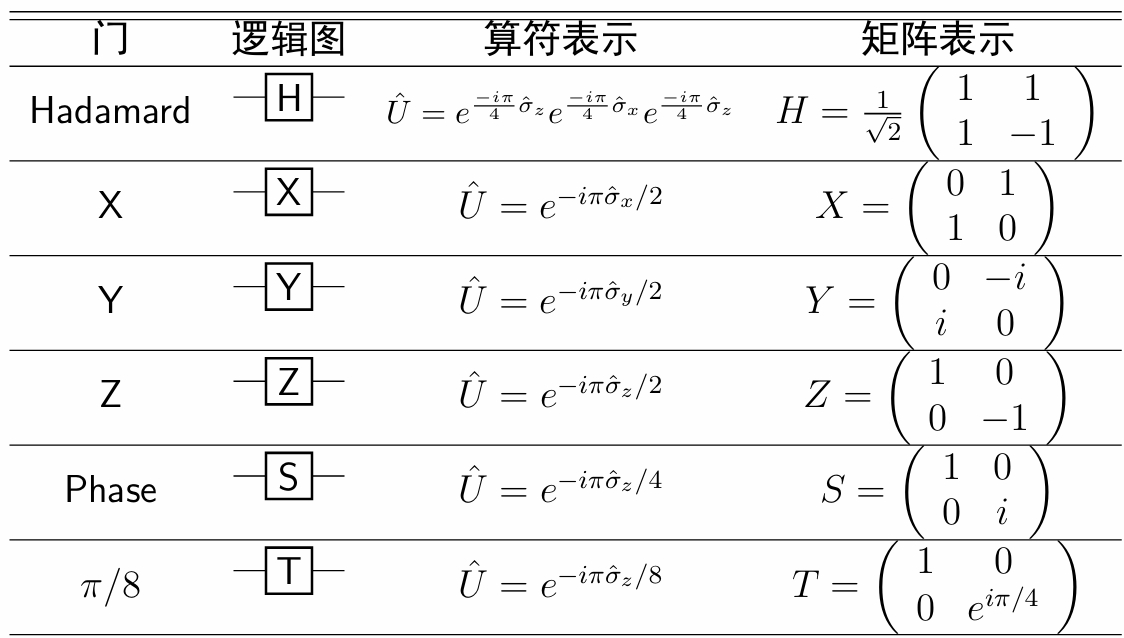
\includegraphics[width=0.8\textwidth]{figures/onedoor.png}
\end{figure}
\textbf{1. Hadamard门(H门)}

\begin{center}
     \begin{quantikz}
          \qw & \gate{H} & \qw \\
     \end{quantikz}
\end{center}


矩阵表示:
     \[
     H = \frac{1}{\sqrt{2}} \begin{pmatrix} 1 & 1 \\ 1 & -1 \end{pmatrix}
     \]

Hadamard门简称H门。H门作用在单量子比特上,将基态\(|0\rangle\)变成\((|0\rangle+|1\rangle)/\sqrt{2}\),将\(|1\rangle\)变成\((|0\rangle-|1\rangle)/\sqrt{2}\),即
     \[
     H|0\rangle = \frac{1}{\sqrt{2}} (|0\rangle + |1\rangle)
     \]
     \[
     H|1\rangle = \frac{1}{\sqrt{2}} (|0\rangle - |1\rangle)
     \]

H门通常用作以下用途:
1. 基变换
2. 将多个量子比特的初态制备为等权叠加态\( H^{\otimes n} \) 作用在零态 \( |0\rangle^{\otimes n} \) 上能够产生等权叠加态\( \frac{1}{\sqrt{2^n}} \sum_{x \in \{0,1\}^n} |x\rangle \)即从零态得到 \( 2^n \) 个态的叠加态。


\textbf{2. Pauli-X门(X门)}

\begin{center}
     \begin{quantikz}
          \qw & \gate{X} & \qw \\
     \end{quantikz}
\end{center}



矩阵表示:
     \[
     X = \begin{pmatrix} 0 & 1 \\ 1 & 0 \end{pmatrix}
     \]

 类似于经典计算中的NOT门,将 \(|0\rangle\) 变为 \(|1\rangle\),将 \(|1\rangle\) 变为 \(|0\rangle\)。
     \[
     X|0\rangle = |1\rangle
     \]
     \[
     X|1\rangle = |0\rangle
     \]

\textbf{3. Pauli-Y门(Y门)}

\begin{center}
     \begin{quantikz}
          \qw & \gate{Y} & \qw \\
     \end{quantikz}
\end{center}


矩阵表示:
     \[
     Y = \begin{pmatrix} 0 & -i \\ i & 0 \end{pmatrix}
     \]
     
类似于X门,但带有相位变化。
     \[
     Y|0\rangle = i|1\rangle
     \]
     \[
     Y|1\rangle = -i|0\rangle
     \]

\textbf{4. Pauli-Z门(Z门)}

\begin{center}
     \begin{quantikz}
          \qw & \gate{Z} & \qw \\
     \end{quantikz}
\end{center}


矩阵表示:
     \[
     Z = \begin{pmatrix} 1 & 0 \\ 0 & -1 \end{pmatrix}
     \]

对量子位的相位进行变化,但不改变其概率幅。
     \[
     Z|0\rangle = |0\rangle
     \]
     \[
     Z|1\rangle = -|1\rangle
     \]

\textbf{5. Phase门(S门)}

\begin{center}
     \begin{quantikz}
          \qw & \gate{S} & \qw \\
     \end{quantikz}
\end{center}


矩阵表示:
     \[
     S = \begin{bmatrix} 1 & 0 \\ 0 & i \end{bmatrix} = \begin{bmatrix} 1 & 0 \\ 0 & e^{i(\pi/2)} \end{bmatrix}
     \]

S门相当于绕布洛赫球z轴逆时针旋转 \(\pi/2\) 角度。布洛赫球上任一量子态 \(|\psi\rangle = \cos\frac{\theta}{2}|0\rangle + e^{i\varphi}\sin\frac{\theta}{2}|1\rangle\),其中 \(e^{i\varphi}\) 是相对相位,\(\varphi\) 是相位角。S门作用后,相位角由 \(\varphi\) 变为 \(\varphi + \pi/2\)。

对于任意量子态\(|\psi\rangle = \alpha|0\rangle + \beta|1\rangle\),S门作用后得到的新的量子态为
     \[
     S|\psi\rangle = \begin{bmatrix} 1 & 0 \\ 0 & i \end{bmatrix} \begin{bmatrix} \alpha \\ \beta \end{bmatrix} = \alpha|0\rangle + i\beta|1\rangle
     \]

\textbf{6. \(\pi/8\)门(T门)}

\begin{center}
     \begin{quantikz}
          \qw & \gate{T} & \qw \\
     \end{quantikz}
\end{center}


矩阵表示:
     \[
     T = \begin{bmatrix} 1 & 0 \\ 0 & e^{i(\pi/4)} \end{bmatrix} 
     \]

 T门相当于绕布洛赫球z轴逆时针旋转 \(\pi/4\) 角度,有时也称之为 \(\pi/8\) 门。
     \[ 
     T = \begin{bmatrix} 1 & 0 \\ 0 & e^{i(\pi/4)} \end{bmatrix} = e^{i(\pi/8)} \begin{bmatrix} e^{-i(\pi/8)} & 0 \\ 0 & e^{i(\pi/8)} \end{bmatrix} 
     \]

上式方括号外的 \(e^{i(\pi/8)}\) 对T门作用后的结果观测不起作用。将T门作用两次等于作用一次S门,即 \(S = TT\)。

 T门作用在任意量子态 \(|\psi\rangle = \alpha|0\rangle + \beta|1\rangle\) 上,得到的新的量子态为
     \[ 
     T|\psi\rangle = \begin{bmatrix} 1 & 0 \\ 0 & e^{i(\pi/4)} \end{bmatrix} \begin{bmatrix} \alpha \\ \beta \end{bmatrix} = \begin{bmatrix} \alpha \\ e^{i(\pi/4)}\beta \end{bmatrix} = \alpha|0\rangle + e^{i(\pi/4)}\beta|1\rangle 
     \] 

\subsubsection{多位门}

\textbf{1. 受控非门(CNOT门)}
\begin{center}
     \begin{quantikz}
          \qw & \ctrl{1} & \qw \\
          \qw & \targ{} & \qw
      \end{quantikz}
\end{center}
受控非门又称CX门或CNOT门,为双量子比特门,其中一个输入为控制量子比特,另一个输入为目标量子比特。当控制量子比特为 \(|1\rangle\) 时,目标量子比特执行X门操作,否则保持不变。

矩阵表示(高位为控制量子比特):
     \[
     \text{CNOT} = \begin{pmatrix} 1 & 0 & 0 & 0 \\ 0 & 1 & 0 & 0 \\ 0 & 0 & 0 & 1 \\ 0 & 0 & 1 & 0 \end{pmatrix}
     \]

作用效果:
     \[
     \text{CNOT}(|00\rangle) = |00\rangle
     \]
     \[
     \text{CNOT}(|01\rangle) = |01\rangle
     \]
     \[
     \text{CNOT}(|10\rangle) = |11\rangle
     \]
     \[
     \text{CNOT}(|11\rangle) = |10\rangle
     \]

\textbf{2. 互换门(SWAP门)}
\begin{center}
     \begin{quantikz}
         \qw & \swap{1} & \qw \\
         \qw & \targX{} & \qw
     \end{quantikz}    
 \end{center}

矩阵表示:
\[
\text{SWAP} = \begin{bmatrix}
1 & 0 & 0 & 0 \\
0 & 0 & 1 & 0 \\
0 & 1 & 0 & 0 \\
0 & 0 & 0 & 1
\end{bmatrix}
\]

对于任意两个量子比特的组合状态,如\(|00\rangle\)、\(|01\rangle\)、\(|10\rangle\)和\(|11\rangle\),SWAP门将分别使它们变为\(|00\rangle\)、\(|10\rangle\)、\(|01\rangle\)和\(|11\rangle\)。SWAP门会交换量子态\(|01\rangle\)和\(|10\rangle\)的状态,而量子态\(|00\rangle\)和\(|11\rangle\)保持不变。

\textbf{3.控制控制非门(Toffoli门)}

\begin{center}
     \begin{quantikz}
      \qw   & \ctrl{1} & \qw \\
      \qw   & \ctrl{1} & \qw \\
      \qw   & \targ{}    & \qw \\
     \end{quantikz}    
 \end{center}

Toffoli门,也称为控制控制非门(Controlled-Controlled-NOT,简称CCNOT),是一种三比特量子门。这种门有两个控制位和一个目标位。当两个控制位都为1时,Toffoli门会对目标位执行NOT操作,即翻转目标位的量子态;如果任一控制位为0,则目标位保持不变。Toffoli门的矩阵表示为一个8×8的矩阵,作用于三比特量子态。

当 \(|q_2 q_1 q_0\rangle\) 中的 \(q_0\) 和 \(q_1\) 为控制量子比特,\(q_2\) 为目标量子比特时,其矩阵表示为:
\[ \text{CCX}_{q_0, q_1, q_2} = I \otimes I \otimes |0\rangle\langle 0| + \text{CX}_{q_1, q_2} \otimes |1\rangle\langle 1| \]

\[ = \begin{bmatrix} 1 & 0 & 0 & 0 & 0 & 0 & 0 & 0 \\ 0 & 1 & 0 & 0 & 0 & 0 & 0 & 0 \\ 0 & 0 & 1 & 0 & 0 & 0 & 0 & 0 \\ 0 & 0 & 0 & 0 & 0 & 0 & 0 & 1 \\ 0 & 0 & 0 & 0 & 1 & 0 & 0 & 0 \\ 0 & 0 & 0 & 0 & 0 & 1 & 0 & 0 \\ 0 & 0 & 0 & 0 & 0 & 0 & 1 & 0 \\ 0 & 0 & 0 & 1 & 0 & 0 & 0 & 0 \end{bmatrix} \]

\subsection{量子线路}
量子线路是实现量子算法的基础。量子线路通过一系列量子门来操作量子位,这些量子位是量子计算的基本单元,可以处于叠加态和纠缠态。
\begin{define}{量子线路(Quantum Circuit)}
     量子线路(Quantum Circuit),也称为量子电路或量子门电路,是量子计算中用于描述量子算法的一种图形化表示方法。它类似于经典计算中的逻辑电路,但专门用于处理量子信息。
\end{define}
量子线路的一个例子:
\begin{center}
     \begin{quantikz}
          \lstick{$\ket{0}$} && \ctrl{1} & \targ{} & \swap{1} & \ctrl[vertical
          wire=c]{2} &&\\
          \lstick{$\ket{0}$} && \control{} & \ctrl[open]{-1} & \targX{} && \gate{X} &\\
          \lstick{$\ket{0}$} &&&& \gate{U} & \meter{} \wire[u][1]{c}
     \end{quantikz}  
\end{center}

\subsection{量子算法}
量子算法是利用量子计算原理进行的计算方法,它能够在特定问题上比经典算法更高效地解决复杂计算任务。与传统计算机使用的经典比特不同,量子比特可以同时处于多种状态,利用叠加和纠缠现象,使得量子计算机能够在进行大规模计算时展现出超越经典计算机的潜力。具体来说,许多需要指数级时间才能解决的问题,在量子算法的帮助下,可以在多项式时间内完成。例如,Shor算法能够有效地分解大整数,从而在加密领域带来革命性的影响。
\begin{define}{量子算法}
    量子算法是运行在量子计算机上的算法,利用量子的特性,如态叠加、量子纠缠等,来解决特定问题。与经典算法相比,量子算法在某些情况下能够显著提高计算速度和效率,解决一些经典计算机难以解决的问题。
\end{define}



